%% ============================================================
%%  Indoor Wayfinding System -- Dissertation Technical Report
%%  Compile with: pdflatex (Overleaf default engine)
%%  No external images -- all figures are pure TikZ
%% ============================================================
\documentclass[12pt,a4paper]{article}

%% -- Encoding (MUST be first) --------------------------------
\usepackage[utf8]{inputenc}
\usepackage[T1]{fontenc}

%% -- Layout & typography ------------------------------------
\usepackage[margin=2.5cm]{geometry}
\usepackage{lmodern}
\usepackage{microtype}
\usepackage{parskip}
\usepackage{setspace}
\onehalfspacing

%% -- Section headings ----------------------------------------
\usepackage{titlesec}
\titleformat{\section}   {\large\bfseries}  {\thesection.}{0.6em}{}
\titleformat{\subsection}{\normalsize\bfseries}{\thesubsection}{0.5em}{}
\titleformat{\subsubsection}{\normalsize\itshape}{\thesubsubsection}{0.4em}{}

%% -- Tables & lists ------------------------------------------
\usepackage{booktabs}
\usepackage{array}
\usepackage{enumitem}

%% -- Floats & captions --------------------------------------
\usepackage{float}
\usepackage{caption}
\usepackage{subcaption}
\captionsetup{font=small, labelfont=bf, width=0.92\linewidth,
              justification=justified, skip=6pt}

%% -- Colour --------------------------------------------------
\usepackage{xcolor}
\definecolor{cBlue}  {HTML}{DBEAFE}
\definecolor{cGreen} {HTML}{D1FAE5}
\definecolor{cYellow}{HTML}{FEF3C7}
\definecolor{cPurple}{HTML}{EDE9FE}
\definecolor{cRed}   {HTML}{FEE2E2}
\definecolor{cSlate} {HTML}{F1F5F9}
\definecolor{cDark}  {HTML}{1E293B}

%% -- TikZ ----------------------------------------------------
\usepackage{tikz}
\usetikzlibrary{shapes.geometric, arrows.meta, positioning,
                fit, backgrounds, calc}

%% Shared node styles (no parametrised args -- safer for pdflatex)
\tikzset{
  blk/.style  = {rectangle, draw=gray!60, rounded corners=3pt,
                 minimum height=0.65cm, text width=#1,
                 align=center, font=\scriptsize, fill=cSlate},
  blk/.default = 2.4cm,
  dec/.style  = {diamond, draw=gray!60, aspect=2.0,
                 minimum height=0.65cm, text width=2.0cm,
                 align=center, font=\scriptsize, fill=cYellow},
  arr/.style  = {->, >=Stealth, semithick},
  darr/.style = {<->, >=Stealth, semithick, dashed},
}

%% -- Hyperlinks ----------------------------------------------
\usepackage{hyperref}
\hypersetup{colorlinks=true, linkcolor=blue!55!black,
            urlcolor=blue!55!black, citecolor=green!40!black}

%% ============================================================
\title{\textbf{Indoor Grid-Based Wayfinding System}\\[4pt]
       \large Technical Report: Methodology, Features, and\\
       RAG-Based Query Framework Integration}
\author{Dissertation Project}
\date{March 2026}
%% ============================================================

\begin{document}
\maketitle
\tableofcontents
\newpage

%% ============================================================
\begin{abstract}
\noindent
This report describes the design, implementation, and user experience of an
indoor wayfinding web application for multi-floor buildings. The system combines
a visual map editor, a grid-based Dijkstra shortest-path engine, and a real-time
localisation layer built on Pedestrian Dead Reckoning (PDR) and QR-code anchor
correction. Multi-floor navigation is supported through stair-cell detection
with user-confirmation prompts. This report also introduces the integration
design for a Retrieval-Augmented Generation (RAG) query framework that resolves
natural-language location queries to grid coordinates, routing the user to the
matched destination automatically. The RAG pipeline runs entirely on local
hardware using a multilingual embedding model, FAISS vector search, a
cross-encoder re-ranker, and a compact open-source LLM.
\end{abstract}

%% ============================================================
\section{Introduction}
\label{sec:intro}
%% ============================================================

Indoor navigation presents challenges not present in outdoor settings: GPS
signals are unavailable inside buildings, floor plans change over time, and
users need real-time positional feedback without dedicated hardware
infrastructure. This project addresses these challenges through a browser-based
wayfinding application that runs on any HTTPS-capable device, including mobile
phones, requiring no native app installation.

The system is built around a \textbf{25$\times$25 cell grid} per floor, with up
to ten independently configurable floors. Each grid cell is classified as one of
four types: \emph{open}, \emph{wall}, \emph{door}, or \emph{stair}. The
application provides two primary modes of operation:

\begin{enumerate}[noitemsep]
  \item \textbf{Map-editor mode} -- for building administrators to design and
    maintain floor plans using paint, stamp, and selection tools.
  \item \textbf{Navigation mode} -- for end users to locate themselves and
    route to a destination cell in real time using PDR and QR anchors.
\end{enumerate}

A planned extension integrates a \textbf{RAG-based query framework} so that
users can describe a destination in plain language (e.g., \textit{``Where is
the registrar's office?''}) and have it resolved automatically to a grid
coordinate, which the routing engine uses as the destination.

%% ============================================================
\section{System Architecture}
\label{sec:arch}
%% ============================================================

The application is a single-page web app served over HTTPS, implemented in
vanilla JavaScript (ES2020) with no runtime framework dependencies. The codebase
is divided into four modules with distinct responsibilities, shown in
Table~\ref{tab:modules}.

\begin{table}[H]
\centering
\caption{Module responsibilities.}
\label{tab:modules}
\small
\begin{tabular}{@{}ll@{}}
\toprule
\textbf{Module} & \textbf{Responsibility} \\
\midrule
\texttt{app.js}      & State machine, event handling, UI orchestration \\
\texttt{nav.js}      & PDR, compass EMA, QR scanning, position updates \\
\texttt{renderer.js} & Canvas drawing: grid, path, overlays, ghost previews \\
\texttt{data.js}     & Node graph, stamp patterns, presets, localStorage \\
\bottomrule
\end{tabular}
\end{table}

Figure~\ref{fig:arch} shows the runtime module relationships and their
connections to the device hardware layer.

\begin{figure}[H]
\centering
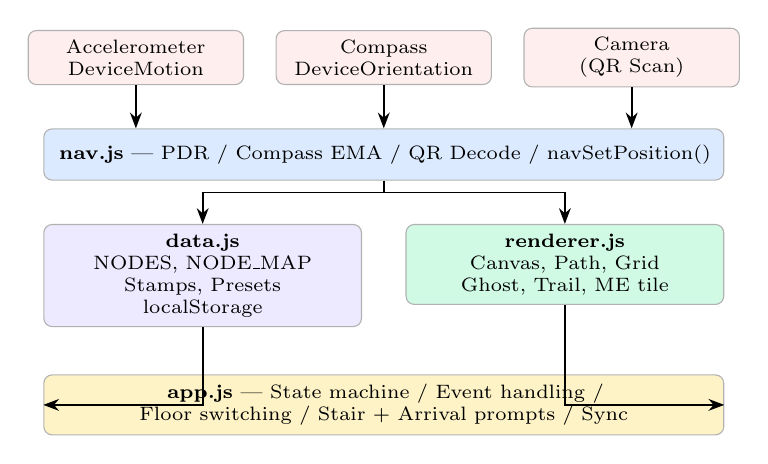
\begin{tikzpicture}[node distance=0.45cm and 0.55cm]

  %% --- Device layer ---
  \node[blk=2.5cm, fill=cRed!60]  (accel)
        {Accelerometer\\DeviceMotion};
  \node[blk=2.5cm, fill=cRed!60, right=0.4cm of accel] (gyro)
        {Compass\\DeviceOrientation};
  \node[blk=2.5cm, fill=cRed!60, right=0.4cm of gyro]  (cam)
        {Camera\\(QR Scan)};

  %% --- nav.js ---
  \node[blk=8.4cm, fill=cBlue,
        below=0.55cm of gyro] (nav)
        {\textbf{nav.js} --- PDR / Compass EMA / QR Decode / navSetPosition()};

  %% --- data.js and renderer.js side by side ---
  \node[blk=3.8cm, fill=cPurple,
        below=0.55cm of nav, xshift=-2.3cm] (data)
        {\textbf{data.js}\\NODES, NODE\_MAP\\Stamps, Presets\\localStorage};

  \node[blk=3.8cm, fill=cGreen,
        below=0.55cm of nav, xshift=2.3cm]  (rend)
        {\textbf{renderer.js}\\Canvas, Path, Grid\\Ghost, Trail, ME tile};

  %% --- app.js ---
  \node[blk=8.4cm, fill=cYellow,
        below=0.6cm of data, xshift=2.3cm]  (app)
        {\textbf{app.js} --- State machine / Event handling /
         Floor switching / Stair + Arrival prompts / Sync};

  %% --- Arrows ---
  \draw[arr] (accel.south) -- ++(0,-0.25) -| (nav.north -| accel);
  \draw[arr] (gyro.south)  -- (nav.north);
  \draw[arr] (cam.south)   -- ++(0,-0.25) -| (nav.north -| cam);

  \draw[arr] (nav.south) -- ++(0,-0.15) -| (data.north);
  \draw[arr] (nav.south) -- ++(0,-0.15) -| (rend.north);

  \draw[arr] (data.south) |- (app.west);
  \draw[arr] (rend.south) |- (app.east);

\end{tikzpicture}
\caption{System module architecture. Device sensors feed \texttt{nav.js}, which
computes updated positions and notifies \texttt{data.js} (graph) and
\texttt{renderer.js} (canvas). \texttt{app.js} orchestrates all state
transitions and persists grid state to \texttt{localStorage}.}
\label{fig:arch}
\end{figure}

%% ============================================================
\section{Map Editor and Grid System}
\label{sec:editor}
%% ============================================================

\subsection{Cell Type System}

Every cell carries a \texttt{cellType} property from the set
$\{\textit{open},\,\textit{wall},\,\textit{door},\,\textit{stair}\}$.
The boolean \texttt{wall} flag used by the pathfinding engine is derived as
\texttt{wall = (cellType === `wall')}, ensuring backward compatibility with
older saves that stored only a boolean. Cell types render with distinct colours
to aid map editing (Table~\ref{tab:celltypes}).

\begin{table}[H]
\centering
\caption{Cell types and their visual and traversal properties.}
\label{tab:celltypes}
\small
\begin{tabular}{@{}llll@{}}
\toprule
\textbf{Type} & \textbf{Colour} & \textbf{Traversable} & \textbf{Special} \\
\midrule
Open  & White              & Yes & --- \\
Wall  & Dark slate         & No  & Blocks routing \\
Door  & Amber              & Yes & --- \\
Stair & Violet             & Yes & Triggers floor-switch logic \\
\bottomrule
\end{tabular}
\end{table}

\subsection{Paint Brush Tool}

In \emph{Wall Mode} the user selects a paint type (Wall / Door / Stair / Erase)
and clicks or drags across the grid. Clicking a cell that already carries the
active type erases it to \emph{open}. Each continuous drag gesture is
recorded as a single undo step.

\subsection{Stamp Tool}

The stamp editor allows administrators to design reusable $n{\times}n$ patterns
(configurable from 2 to 15, default 5). Cells in the editor are painted with
the active paint type. When a stamp is placed on the main grid, \emph{open}
cells in the pattern are transparent -- they do not overwrite existing
content -- so only walls, doors, and stairs from the pattern are applied.

Named stamps are logged in a searchable \emph{catalogue} with jump-to
navigation. Frequently-used patterns can be saved as \emph{presets} and
recalled in future sessions.

\subsection{Selection and Region Manipulation}

In \emph{Select Mode} the user drags to define a rectangular region. A toolbar
offers rotate CW/CCW, lift-and-move (floating ghost dropped on next tap), and
delete. Open cells in a moved pattern are transparent on drop.

\subsection{Multi-Floor Support}

Up to ten independent floors are supported. Switching floors serialises the
current floor's cell-type array into a \texttt{FLOOR\_WALLS} cache and loads
the target floor (blank grid if first visit). The active floor number is
displayed as a watermark on the canvas.

\subsection{Undo / Redo and Persistence}

Every destructive edit pushes a snapshot onto an undo stack (max 50 entries).
Undo/redo is available via toolbar buttons and \texttt{Ctrl+Z} / \texttt{Ctrl+Y}.
Grid state (all floors, stamps, and presets) is written to \texttt{localStorage}
after every edit and optionally pushed to a backend REST endpoint for
cross-device synchronisation.

%% ============================================================
\section{Pathfinding Engine}
\label{sec:path}
%% ============================================================

Routing is computed with \textbf{Dijkstra's algorithm} on a four-connected
adjacency graph. Wall cells are excluded; all other types are traversable with
uniform edge weight 1. The start node is the ME tile and the destination is any
non-wall cell tapped by the user.

The info bar displays step count and an estimated metric distance:
\[
  d \;=\; \textit{steps} \;\times\; \texttt{metresPerCell}
\]
where \texttt{metresPerCell} is calibrated by measuring a known corridor and
dividing its length by the number of cells it spans.

%% ============================================================
\section{Navigation Mode}
\label{sec:nav}
%% ============================================================

\subsection{Pedestrian Dead Reckoning (PDR)}

PDR estimates position by integrating step events and compass headings.
Figure~\ref{fig:pdr} shows the signal-processing pipeline.

\begin{figure}[H]
\centering
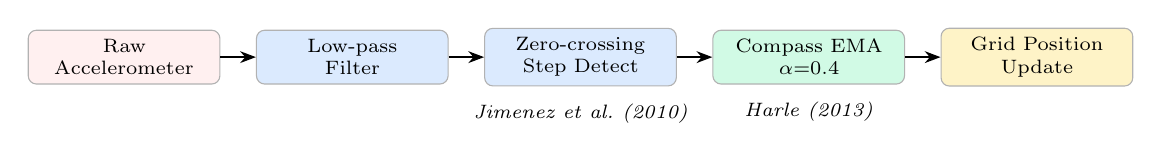
\begin{tikzpicture}[node distance=0.4cm and 0.45cm]

  \node[blk=2.2cm, fill=cRed!50]   (raw) {Raw\\Accelerometer};
  \node[blk=2.2cm, fill=cBlue,   right=of raw]  (lpf) {Low-pass\\Filter};
  \node[blk=2.2cm, fill=cBlue,   right=of lpf]  (zc)  {Zero-crossing\\Step Detect};
  \node[blk=2.2cm, fill=cGreen,  right=of zc]   (hdg) {Compass EMA\\$\alpha{=}0.4$};
  \node[blk=2.2cm, fill=cYellow, right=of hdg]  (pos) {Grid Position\\Update};

  \draw[arr] (raw)--(lpf);
  \draw[arr] (lpf)--(zc);
  \draw[arr] (zc) --(hdg);
  \draw[arr] (hdg)--(pos);

  \node[font=\scriptsize\itshape, below=0.1cm of zc]
        {Jimenez et al.\ (2010)};
  \node[font=\scriptsize\itshape, below=0.1cm of hdg]
        {Harle (2013)};

\end{tikzpicture}
\caption{PDR signal-processing pipeline. Zero-crossing step detection
(Jimenez et al., 2010) is phone-position invariant. Compass heading is smoothed
with an EMA ($\alpha{=}0.4$) for responsive turn tracking (Harle, 2013).}
\label{fig:pdr}
\end{figure}

\paragraph{Step Detection.}
Vertical acceleration is low-pass filtered; a step is registered each time the
signal crosses zero downward (Jimenez et al., 2010). This method is invariant
to how the phone is held -- pocket, hand, or bag.

\paragraph{Heading.}
Compass bearing from the DeviceOrientation API is smoothed with an EMA
($\alpha{=}0.4$). Steps are suppressed until the first valid compass reading
(\texttt{\_compassReady} guard).

\paragraph{Position Update.}
Each step advances the ME tile one cell in the direction of the current
heading, discretised to the nearest 45\textdegree{} for clean grid movement.

\subsection{QR Code Anchor Correction}

PDR accumulates drift over time. Printed QR codes at known locations provide
correction anchors. The QR payload encodes floor, row, and column:

\begin{center}
\ttfamily
GRID:\textlangle floor\textrangle:\textlangle row\textrangle,\textlangle col\textrangle
\end{center}

Figure~\ref{fig:qr} shows the scan-and-correct workflow.

\begin{figure}[H]
\centering
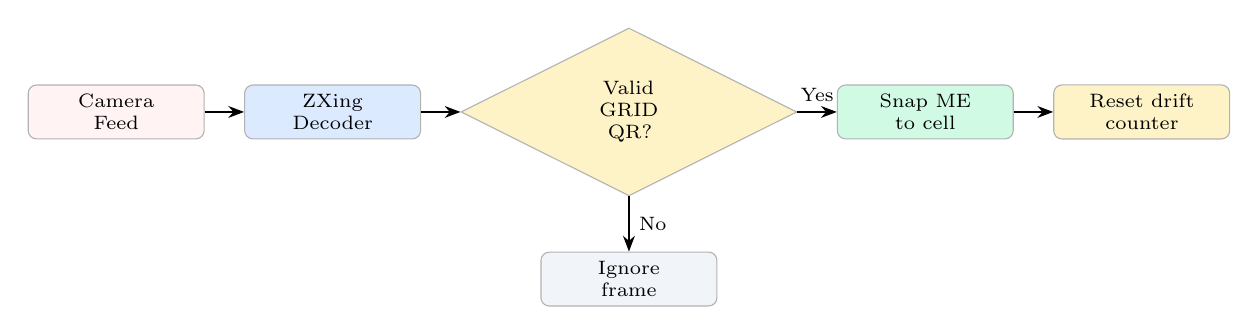
\begin{tikzpicture}[node distance=0.4cm and 0.5cm]

  \node[blk=2.0cm, fill=cRed!40]  (cam)  {Camera\\Feed};
  \node[blk=2.0cm, fill=cBlue,  right=of cam]  (dec)  {ZXing\\Decoder};
  \node[dec,                     right=0.5cm of dec]   (val)
        {Valid\\GRID\\QR?};
  \node[blk=2.0cm, fill=cGreen, right=0.5cm of val]   (snp)  {Snap ME\\to cell};
  \node[blk=2.0cm, fill=cYellow,right=of snp]          (rst)  {Reset drift\\counter};
  \node[blk=2.0cm, fill=cSlate, below=0.7cm of val]   (rej)  {Ignore\\frame};

  \draw[arr] (cam)--(dec);
  \draw[arr] (dec)--(val);
  \draw[arr] (val)-- node[above, font=\scriptsize]{Yes} (snp);
  \draw[arr] (snp)--(rst);
  \draw[arr] (val)-- node[right, font=\scriptsize]{No}  (rej);

\end{tikzpicture}
\caption{QR anchor correction workflow. A successful scan snaps the ME tile to
the encoded cell and floor; the drift counter resets to zero.}
\label{fig:qr}
\end{figure}

\paragraph{Drift Indicator.}
A colour-coded chip shows steps since the last QR fix: green (${\leq}5$),
amber (6--15), red ($>15$). Before the first fix the label shows ``Fix: --''.

\paragraph{QR Generator.}
Administrators generate and download printable QR codes from within the app.
The floor field uses 1-indexed display values (Floor 1 = ground); conversion to
0-indexed internal values occurs at the input/output boundary.

%% ============================================================
\section{Stair Navigation and Arrival Detection}
\label{sec:stair}
%% ============================================================

\subsection{Stair Cell Detection}

When the ME tile moves onto a \texttt{stair} cell, the system checks whether
adjacent floors (floor $\pm$1) have a stair cell at the same grid coordinates,
using the flat array index \texttt{row $\times$ GRID\_COLS + col} against the
\texttt{FLOOR\_WALLS} cache. Figure~\ref{fig:stair} shows the resulting decision
tree.

\begin{figure}[H]
\centering
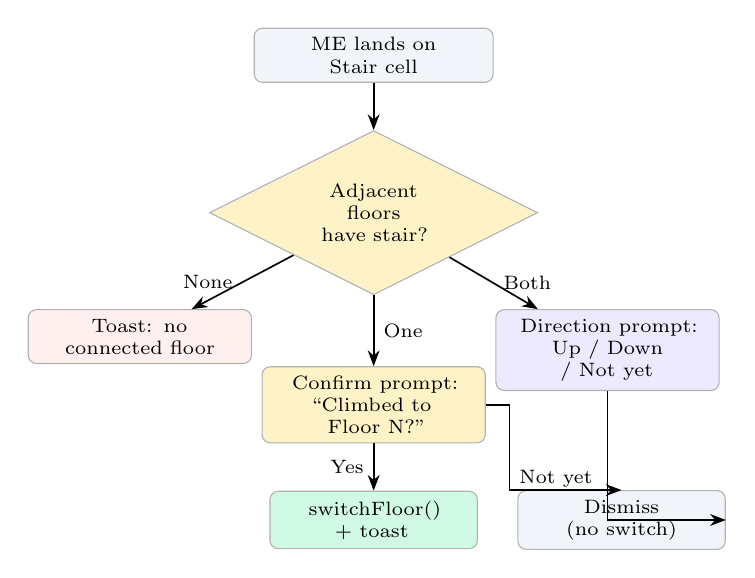
\begin{tikzpicture}[node distance=0.5cm and 0.7cm]

  \node[blk=2.8cm, fill=cSlate]  (land)
        {ME lands on\\Stair cell};

  \node[dec, below=0.6cm of land] (chk)
        {Adjacent\\floors\\have stair?};

  \node[blk=2.6cm, fill=cRed!50,
        below left=0.7cm and 0.5cm of chk]  (none)
        {Toast: no\\connected floor};

  \node[blk=2.6cm, fill=cYellow,
        below=0.9cm of chk]                 (one)
        {Confirm prompt:\\``Climbed to\\Floor N?''};

  \node[blk=2.6cm, fill=cPurple,
        below right=0.7cm and 0.5cm of chk] (both)
        {Direction prompt:\\Up / Down\\/ Not yet};

  \node[blk=2.4cm, fill=cGreen,
        below=0.6cm of one]                 (sw)
        {switchFloor()\\+ toast};

  \node[blk=2.4cm, fill=cSlate,
        right=0.5cm of sw]                  (dis)
        {Dismiss\\(no switch)};

  \draw[arr] (land)--(chk);
  \draw[arr] (chk) -- node[left,  font=\scriptsize]{None} (none);
  \draw[arr] (chk) -- node[right, font=\scriptsize]{One}  (one);
  \draw[arr] (chk) -- node[right, font=\scriptsize]{Both} (both);
  \draw[arr] (one) -- node[left,  font=\scriptsize]{Yes}  (sw);
  \draw[arr] (one.east) -- ++(0.3,0) |- node[right, font=\scriptsize, yshift=4pt]{Not yet} (dis.north);
  \draw[arr] (both.south) |- (dis.east);

\end{tikzpicture}
\caption{Stair navigation decision tree. Single-direction stairs show a
confirmation prompt before switching floors. Bidirectional stairs present an
explicit up/down choice. All prompts auto-dismiss after 8 seconds.}
\label{fig:stair}
\end{figure}

A 2-second cooldown prevents re-firing while the user stands on the same stair
cell. The cooldown key includes the floor index so that a stair encountered
after switching floors correctly re-triggers the logic.

\subsection{Arrival Detection}

After every position update, the ME tile's node ID is compared to the current
destination ID. On a match, a green ``You have arrived!'' banner animates in at
the centre of the screen, auto-dismissing after 4 seconds. The banner is also
hidden when navigation mode is turned off.

%% ============================================================
\section{RAG-Based Query Framework}
\label{sec:rag}
%% ============================================================

\subsection{Motivation}

Users navigating an unfamiliar building know a destination by \emph{name}, not
by grid coordinates. The RAG Query Module bridges this gap: it accepts a
natural-language query (e.g., ``Where is Room 204?''), retrieves the most
relevant entry from a curated building knowledge base, and resolves the answer
to a grid coordinate. \texttt{app.js} then calls \texttt{handleCellTap(row,
col)} to set the routing destination automatically.

The module is based on a fully local Advanced RAG architecture validated for
domain-specific question answering. It is adapted here for building-information
retrieval.

\subsection{Architecture Overview}

The six-stage pipeline, illustrated in Figure~\ref{fig:rag}, runs entirely on
local hardware, requiring no cloud API access. Total GPU memory usage is
approximately 3.7 GB, within the limits of consumer-grade hardware.

\begin{figure}[H]
\centering
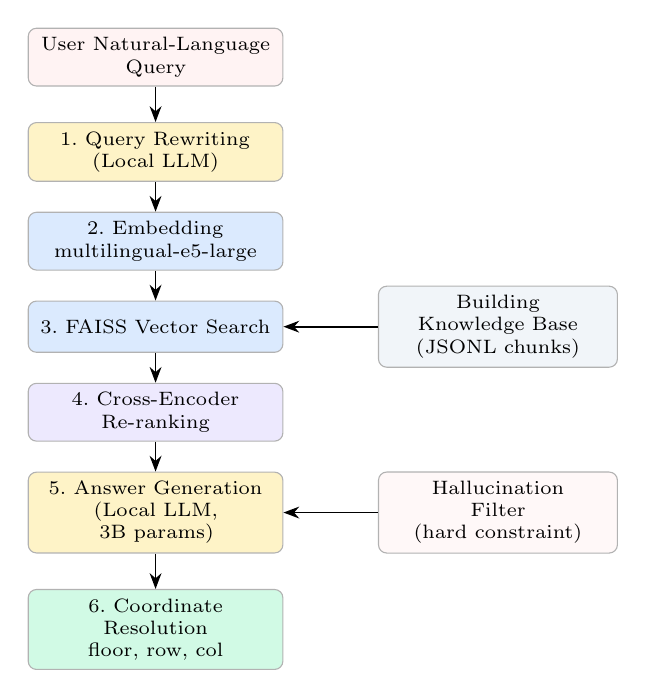
\begin{tikzpicture}[node distance=0.38cm]

  %% Main pipeline (left column)
  \node[blk=3.0cm, fill=cRed!40]   (q)
        {User Natural-Language\\Query};
  \node[blk=3.0cm, fill=cYellow, below=0.45cm of q]   (rw)
        {1.\ Query Rewriting\\(Local LLM)};
  \node[blk=3.0cm, fill=cBlue,   below=0.38cm of rw]  (emb)
        {2.\ Embedding\\multilingual-e5-large};
  \node[blk=3.0cm, fill=cBlue,   below=0.38cm of emb] (ret)
        {3.\ FAISS Vector Search};
  \node[blk=3.0cm, fill=cPurple, below=0.38cm of ret] (rrk)
        {4.\ Cross-Encoder\\Re-ranking};
  \node[blk=3.0cm, fill=cYellow, below=0.38cm of rrk] (gen)
        {5.\ Answer Generation\\(Local LLM, 3B params)};
  \node[blk=3.0cm, fill=cGreen,  below=0.45cm of gen] (out)
        {6.\ Coordinate Resolution\\floor, row, col};

  %% Right column
  \node[blk=2.8cm, fill=cSlate,
        right=1.2cm of ret]  (kb)
        {Building\\Knowledge Base\\(JSONL chunks)};
  \node[blk=2.8cm, fill=cRed!25,
        right=1.2cm of gen]  (flt)
        {Hallucination\\Filter\\(hard constraint)};

  %% Arrows
  \draw[arr] (q)  --(rw);
  \draw[arr] (rw) --(emb);
  \draw[arr] (emb)--(ret);
  \draw[arr] (ret)--(rrk);
  \draw[arr] (rrk)--(gen);
  \draw[arr] (gen)--(out);
  \draw[arr] (kb.west)  -- (ret.east);
  \draw[arr] (flt.west) -- (gen.east);

\end{tikzpicture}
\caption{Fully local RAG pipeline for the Query Module. All inference runs on
consumer-grade hardware. The hallucination filter removes any location
identifier in the answer that does not appear in the retrieved chunks.}
\label{fig:rag}
\end{figure}

\subsection{Pipeline Stages}

\paragraph{Stage 1 -- Query Rewriting.}
A locally hosted compact LLM normalises the user's raw query into a
well-formed interrogative statement, expanding shorthand and translating
informal phrasing. A fallback guard discards rewrites shorter than five words
and substitutes the original query.

\paragraph{Stage 2 -- Embedding.}
The rewritten query is encoded by \textbf{multilingual-e5-large}. Multilingual
support handles code-switched queries common in multilingual environments.

\paragraph{Stage 3 -- FAISS Vector Search.}
Embeddings are searched against a FAISS index of building knowledge chunks using
exact inner-product search. Each chunk is annotated with a grid coordinate
(floor, row, column).

\paragraph{Stage 4 -- Cross-Encoder Re-ranking.}
A \textbf{BAAI/bge-reranker-base} cross-encoder jointly encodes each
query-chunk pair for more accurate relevance scoring, reducing noise from
bi-encoder approximate search (Glass et al., 2022).

\paragraph{Stage 5 -- Answer Generation.}
Top-ranked chunks are assembled into a grounded prompt passed to the locally
hosted 3B-parameter LLM via Ollama. A post-processing filter then enforces
groundedness: any location identifier in the output that does not appear in the
retrieved chunks is removed before the answer is returned.

\paragraph{Stage 6 -- Coordinate Resolution.}
The structured answer includes the grid coordinate of the matched location.
\texttt{app.js} parses this and calls \texttt{handleCellTap(row, col)}, setting
the destination without any further user action.

\subsection{Knowledge Base Construction}

The building knowledge base is curated offline by administrators. Each JSONL
record contains a natural-language description, a 0-indexed floor number, grid
coordinates (row, col), and searchable tags. Adding or updating entries requires
only re-running the FAISS indexing script -- no model retraining is needed.

\subsection{Evaluation Framework}

System quality is assessed across four tiers:

\begin{enumerate}[label=\textbf{Tier \arabic*.}, leftmargin=2.5cm, noitemsep]
  \item \textbf{Retrieval Quality} -- Recall@k, Precision@k, MRR, NDCG@k
        against ground-truth coordinate annotations.
  \item \textbf{Generation Quality} -- ROUGE-L, METEOR, BERTScore (F1),
        SBERT cosine similarity against gold descriptions.
  \item \textbf{RAG Faithfulness} -- RAGAS metrics: Faithfulness, Answer
        Correctness, Context Precision, Context Recall.
  \item \textbf{System Performance} -- Mean response latency from query
        submission to coordinate output.
\end{enumerate}

Statistical significance across configuration comparisons is assessed with
paired Wilcoxon signed-rank tests ($\alpha = 0.05$).

%% ============================================================
\section{User Experience}
\label{sec:ux}
%% ============================================================

\subsection{App Mode State Machine}

The application operates as a strict modal state machine: at most one mode is
active at a time. Entering a mode automatically deactivates any conflicting
active mode. Figure~\ref{fig:ux} shows the full state transition diagram.

\begin{figure}[H]
\centering
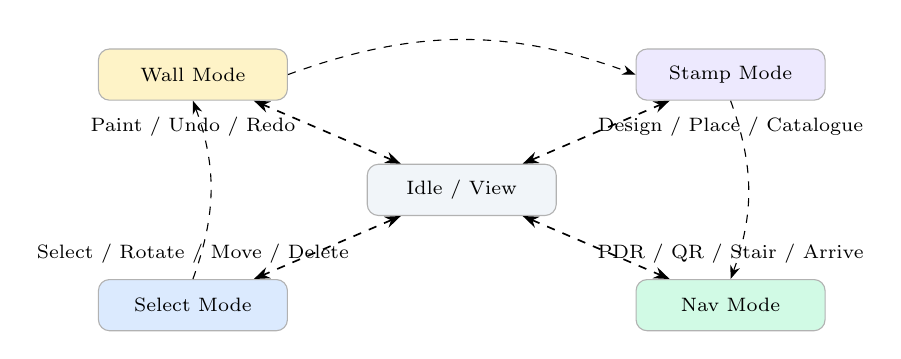
\begin{tikzpicture}[
  st/.style={rectangle, draw=gray!60, rounded corners=4pt, fill=#1,
             minimum width=2.4cm, minimum height=0.65cm,
             align=center, font=\scriptsize},
  st/.default=cSlate,
  node distance=0.8cm and 1.1cm,
]
  \node[st=cSlate]   (idle)  {Idle / View};

  \node[st=cYellow,  above left=0.8cm  and 1.0cm of idle] (wall)
        {Wall Mode};
  \node[st=cPurple,  above right=0.8cm and 1.0cm of idle] (stp)
        {Stamp Mode};
  \node[st=cBlue,    below left=0.8cm  and 1.0cm of idle] (sel)
        {Select Mode};
  \node[st=cGreen,   below right=0.8cm and 1.0cm of idle] (nav)
        {Nav Mode};

  \draw[darr] (idle)--(wall);
  \draw[darr] (idle)--(stp);
  \draw[darr] (idle)--(sel);
  \draw[darr] (idle)--(nav);

  %% Cross-mode deactivation (dashed single-direction)
  \draw[->, >=Stealth, dashed, bend left=20] (wall.east) to (stp.west);
  \draw[->, >=Stealth, dashed, bend left=20] (stp.south) to (nav.north);
  \draw[->, >=Stealth, dashed, bend right=20](sel.north) to (wall.south);

  %% Sub-labels
  \node[font=\scriptsize, below=0.08cm of wall]
        {Paint / Undo / Redo};
  \node[font=\scriptsize, below=0.08cm of stp]
        {Design / Place / Catalogue};
  \node[font=\scriptsize, above=0.08cm of sel]
        {Select / Rotate / Move / Delete};
  \node[font=\scriptsize, above=0.08cm of nav]
        {PDR / QR / Stair / Arrive};

\end{tikzpicture}
\caption{App mode state machine. Dashed arrows indicate automatic mode
deactivation: entering any mode forces conflicting modes off. The Idle state
handles tap-to-route destination setting.}
\label{fig:ux}
\end{figure}

\subsection{Overlay Bar Layout}

The navigation panel, hint bar, paint-type bar, and selection toolbar are
absolutely positioned overlays inside the canvas container. This ensures the
map canvas always fills the full available height regardless of how many bar
rows are visible -- eliminating canvas-shrink issues that arise when overlay
bars participate in the flex layout flow.

\subsection{UI Design Rationale}

\begin{enumerate}[label=\textbf{D\arabic*.}, leftmargin=2cm, noitemsep]
  \item \textbf{No on-screen D-pad.} PDR and QR scanning replace manual
    movement controls on mobile; arrow-key navigation remains available on
    desktop for accessibility.

  \item \textbf{Transparent stamp open-cells.} Open cells in a stamp pattern
    do not overwrite existing content, enabling partial overlay patterns
    (e.g., doorframes) without erasing surrounding walls.

  \item \textbf{Confirmation before floor switch.} Automatic floor switching
    on stair contact was replaced with a confirmation prompt to prevent false
    switches caused by incidental stair-cell contact.

  \item \textbf{1-indexed floor display.} All user-facing floor labels use
    1-indexed values (Floor 1 = ground) to match building signage. Internal
    logic uses 0-indexed values; conversion occurs at the input/output boundary.

  \item \textbf{Drift-aware trust signal.} The drift indicator gives users an
    explicit confidence signal, encouraging proactive QR rescanning when drift
    is high.
\end{enumerate}

%% ============================================================
\section{Feature Summary}
\label{sec:features}
%% ============================================================

Table~\ref{tab:features} provides a complete inventory of implemented features.

\begin{table}[H]
\centering
\caption{Feature inventory of the current working application.}
\label{tab:features}
\small
\renewcommand{\arraystretch}{1.15}
\begin{tabular}{@{}p{3.8cm}p{8.6cm}@{}}
\toprule
\textbf{Feature} & \textbf{Description} \\
\midrule
Cell type system       & Four types: open, wall, door, stair; backward-compatible with boolean saves \\
Paint brush            & Click/drag painting; same-type click erases; one drag = one undo step \\
Stamp tool             & $n{\times}n$ reusable patterns; transparent open cells; rotation \\
Stamp presets          & Save and reload named patterns across sessions \\
Stamp catalogue        & Named placements logged with jump-to navigation \\
Select \& manipulate   & Region select; rotate CW/CCW; lift-and-move; delete \\
Multi-floor support    & Up to 10 independent floor layouts; floor watermark on canvas \\
Undo / Redo            & 50-step history; Ctrl+Z / Ctrl+Y \\
Pathfinding            & Dijkstra shortest path; step count and estimated metres \\
PDR localisation       & Zero-crossing step detection; EMA compass; phone-position invariant \\
QR anchor correction   & Scan to snap position; floor-aware; drift counter reset \\
QR code generator      & Generate and download printable anchor QR codes for any cell \\
Drift indicator        & Green/amber/red trust signal; neutral until first QR fix \\
Stair navigation       & Stair-cell detection; single/bidirectional prompts; 8 s auto-dismiss \\
Arrival detection      & ``You have arrived!'' on destination reach; 4 s auto-dismiss \\
Breadcrumb trail       & Last 10 positions on canvas; fades with age \\
RAG query module       & Natural-language query to grid coordinate; local inference; hallucination filter \\
Grid persistence       & localStorage auto-save; optional server sync \\
Mobile-responsive UI   & Overlay bars; collapsible header; touch targets at least 40 px \\
\bottomrule
\end{tabular}
\end{table}

%% ============================================================
\section{Conclusion}
\label{sec:conclusion}
%% ============================================================

This report has described a complete indoor wayfinding system covering map
editing, multi-floor management, shortest-path routing, real-time PDR and QR
localisation, stair-aware floor switching, and arrival detection. The system
operates entirely in the browser with no native app installation required.

The planned RAG Query Module will allow users to navigate to named destinations
without knowing grid coordinates, combining grid-based precision with natural-
language accessibility. The fully local pipeline ensures that both the
wayfinding engine and the query module operate offline -- an important property
for buildings with limited internet connectivity.

\paragraph{Future Work.}
(1) Calibrate \texttt{metresPerCell} with real corridor measurements and run
PDR evaluation conditions A/B/C/D for dissertation fieldwork.
(2) Populate the building knowledge base with room and facility metadata.
(3) Integrate RAG coordinate-resolution output into the live routing pipeline.
(4) Conduct a user study evaluating wayfinding accuracy and task completion time.

\end{document}
